\documentclass[journal]{IEEEtran}

\usepackage[spanish,es-nodecimaldot,es-noquoting]{babel}
\usepackage[T1]{fontenc}
\usepackage[utf8]{inputenc}
\usepackage{amsmath,amssymb}
\usepackage{graphicx}
\usepackage{booktabs}
\usepackage{multirow}
\usepackage{array}
\usepackage{url}
\usepackage{float}

\graphicspath{{../figuras/}{figuras/}}

\addto\captionsspanish{\renewcommand{\tablename}{Tabla}\renewcommand{\figurename}{Figura}}
\renewcommand{\thetable}{S\arabic{table}}
\renewcommand{\thefigure}{S\arabic{figure}}

\begin{document}

\title{Material suplementario: asistente RAG sobre prensa colombiana e internacional y Bluesky}
\author{Erika Valeria Rivera Jimenez, Julian Guillermo Carrillo Meneses,\\
Carlos Andres Garnica Salazar, Oscar Andres Prieto Moreno}

\maketitle

\section*{Presentaci\'on}

Este suplemento re\'une las tablas y figuras que el cuerpo del art\'iculo referencia como S1 a S6. Se separaron para mantener el cuerpo en 16 p\'aginas; los datos, las corridas y los artefactos son los mismos y se describen en la secci\'on de reproducibilidad del art\'iculo.

\section*{Reordenamiento con bge-m3}

La Tabla~\ref{tab:s1} mide el reordenador en CPU sobre 38 preguntas. El top-5 mantiene el recall y sube el nDCG y el P@1; el top-20 pierde Hit@5 y multiplica la latencia.

\begin{table}[H]
\centering
\footnotesize
\caption{Reordenamiento con bge-m3 (38 preguntas).}
\label{tab:s1}
\begin{tabular}{lrrrrr}
\toprule
Configuraci\'on & Recall & nDCG & P@1 & Hit@5 & p50 \\
\midrule
Denso top-5 & 0,895 & 0,809 & 0,737 & 0,947 & 0,10 s \\
Rerank top-5 & 0,895 & \textbf{0,865} & \textbf{0,868} & \textbf{0,947} & 1,30 s \\
Rerank top-20 & 0,864 & 0,853 & \textbf{0,868} & 0,921 & 5,46 s \\
\bottomrule
\end{tabular}
\end{table}

\section*{Fases 6 y 7}

La Tabla~\ref{tab:s2} resume las variantes de prompt y diversidad probadas sobre 38 preguntas. Ninguna supera a la referencia del top-5 con reranker.

\begin{table}[H]
\centering
\footnotesize
\caption{Fases 6 y 7: variantes probadas sobre 38 preguntas. La referencia es el top-5 con reranker.}
\label{tab:s2}
\resizebox{\columnwidth}{!}{%
\begin{tabular}{lrrrrl}
\toprule
Variante & Recall & nDCG & P@1 & Hit@5 & Decisi\'on \\
\midrule
Top-5 con reranker & \textbf{0,895} & \textbf{0,865} & \textbf{0,868} & \textbf{0,947} & Referencia \\
Rerank top-20 & 0,864 & 0,853 & \textbf{0,868} & 0,921 & Rechazada \\
Filtro por score 0,8 & 0,838 & 0,837 & \textbf{0,868} & 0,921 & Rechazada \\
Filtro por score 0,9 & 0,825 & 0,830 & \textbf{0,868} & 0,921 & Rechazada \\
Expansi\'on de consulta & 0,825 & 0,739 & 0,658 & 0,895 & Rechazada \\
MMR coseno 0,5 & 0,868 & 0,784 & 0,737 & \textbf{0,947} & Rechazada \\
MMR con reranker 0,7 & 0,816 & 0,818 & \textbf{0,868} & 0,921 & Rechazada \\
\bottomrule
\end{tabular}
}
\end{table}

\section*{Conjunto reservado}

La Tabla~\ref{tab:s3} reporta el conjunto reservado de 25 preguntas, congelado antes de evaluar la compuerta. La recuperaci\'on h\'ibrida se eligi\'o despu\'es con ese mismo conjunto, as\'i que las m\'etricas de recuperaci\'on y respuesta son de desarrollo.

\begin{table}[H]
\centering
\footnotesize
\caption{Conjunto reservado: 20 preguntas directas y 5 sin respuesta, congelado antes de ejecutar.}
\label{tab:s3}
\begin{tabular}{lrr}
\toprule
M\'etrica & Valor & Denominador \\
\midrule
Recall@10 & 0,700 & 20 \\
nDCG@10 & 0,612 & 20 \\
P@1 & 0,500 & 20 \\
Hit@5 & 0,650 & 20 \\
Cobertura de span & 0,700 & 20 \\
Entregadas & 19 & 20 \\
Abstenciones en directas & 1 & 20 \\
Cobertura de tokens, entregadas & 17 & 19 \\
Cobertura de tokens, todas & 17 & 20 \\
Con cita & 1,000 & 19 \\
Abstenciones en sin respuesta & 5 & 5 \\
Compuerta rechaza & 5 & 5 \\
Latencia media & 6,2 s & 25 \\
\bottomrule
\end{tabular}
\end{table}

\section*{Inyecci\'on de instrucciones}

La Tabla~\ref{tab:inyeccion} mide E5 sobre 38 preguntas. Gemma2:2b obedeci\'o una de cinco instrucciones y a\~nadi\'o la palabra pedida; los otros dos modelos las ignoraron. La prueba es exploratoria: no cubre el generador final ni demuestra robustez general.

\begin{table}[H]
\centering
\footnotesize
\caption{E5: instrucciones inyectadas en el texto recuperado.}
\label{tab:inyeccion}
\begin{tabular}{lrrr}
\toprule
Modelo & Obedeci\'o & Respondi\'o el hecho & Se abstuvo \\
\midrule
gemma2:2b & 1/5 & 4/5 & 0/5 \\
llama3.2:3b & 0/5 & 5/5 & 0/5 \\
qwen2.5:1.5b & 0/5 & 5/5 & 0/5 \\
\bottomrule
\end{tabular}
\end{table}


\section*{Figuras del an\'alisis exploratorio}

Las Figuras~\ref{fig:s1} a~\ref{fig:s4} muestran la composici\'on por colecci\'on, la relaci\'on rango-frecuencia, los idiomas normalizados y la distribuci\'on de longitud. No cambian las decisiones de dise\~no; los totales citados est\'an en las Tablas I y II del art\'iculo.

\begin{figure*}[t]
\centering
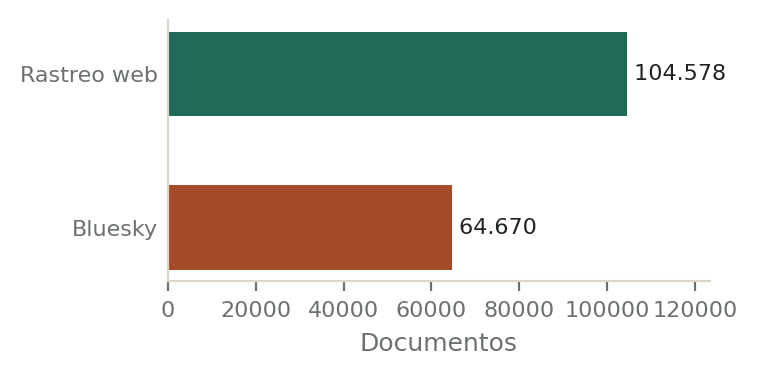
\includegraphics[width=0.8\textwidth]{perfil_colecciones.png}
\caption{Documentos por colecci\'on. Los dos totales coinciden con la Tabla~I del art\'iculo.}
\label{fig:s1}
\end{figure*}


\begin{figure*}[t]
\centering
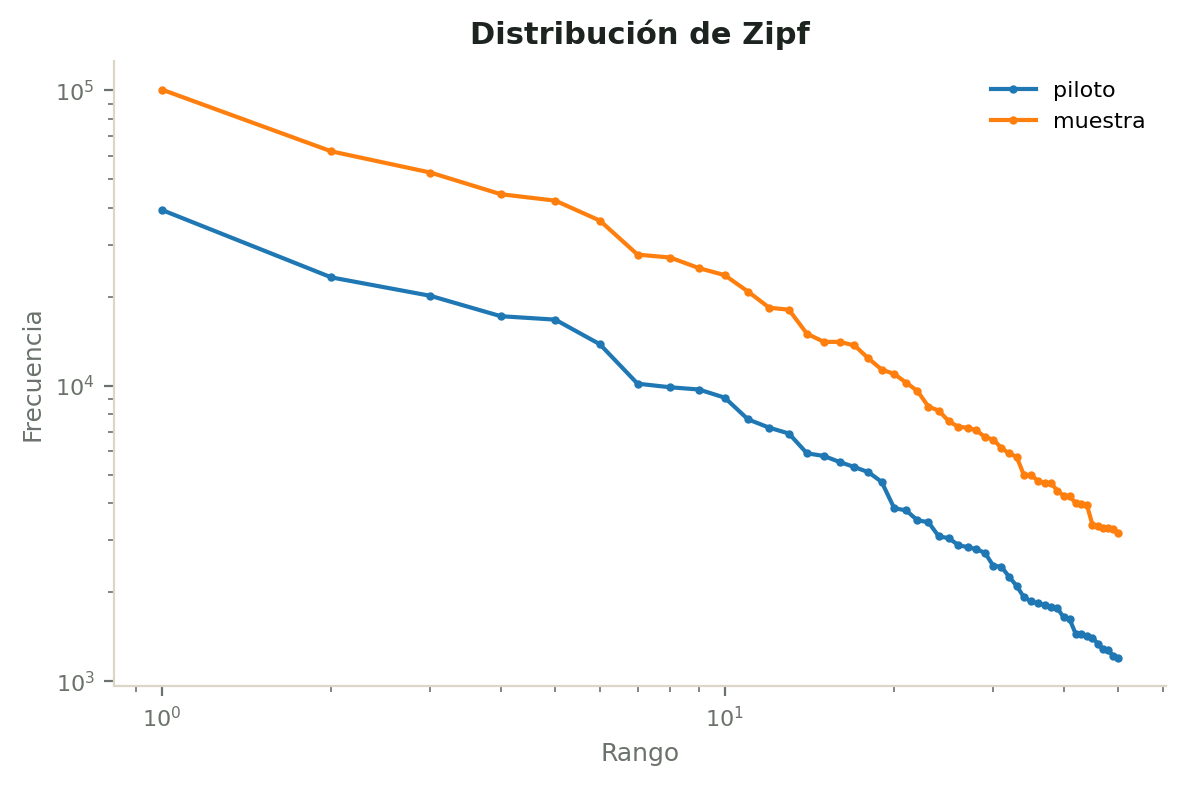
\includegraphics[width=0.8\textwidth]{textometria_zipf.png}
\caption{Rango frente a frecuencia en escala logar\'itmica para el piloto y la muestra. Se muestran los 50 t\'erminos m\'as frecuentes; no se ajusta una recta, la figura solo comprueba la forma de ley de potencia.}
\label{fig:s2}
\end{figure*}


\begin{figure*}[t]
\centering
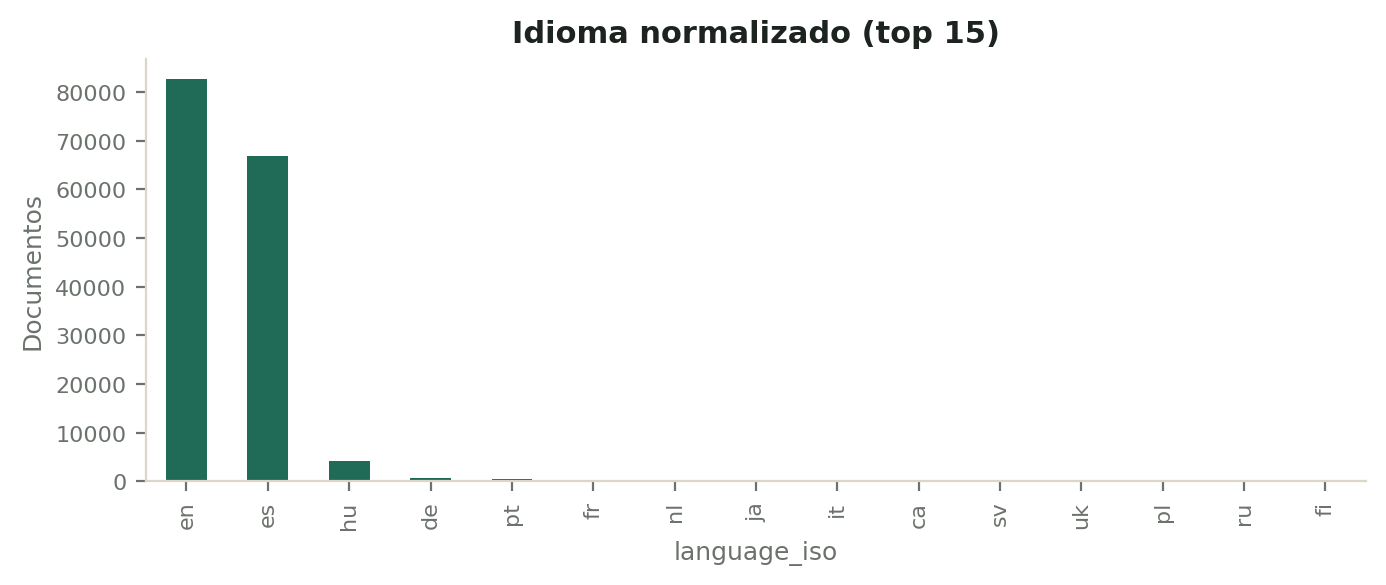
\includegraphics[width=0.8\textwidth]{perfil_idiomas.png}
\caption{Idiomas normalizados m\'as frecuentes (15 primeros). La normalizaci\'on se hace al vuelo; el campo crudo del archivo no se modifica.}
\label{fig:s3}
\end{figure*}


\begin{figure*}[t]
\centering
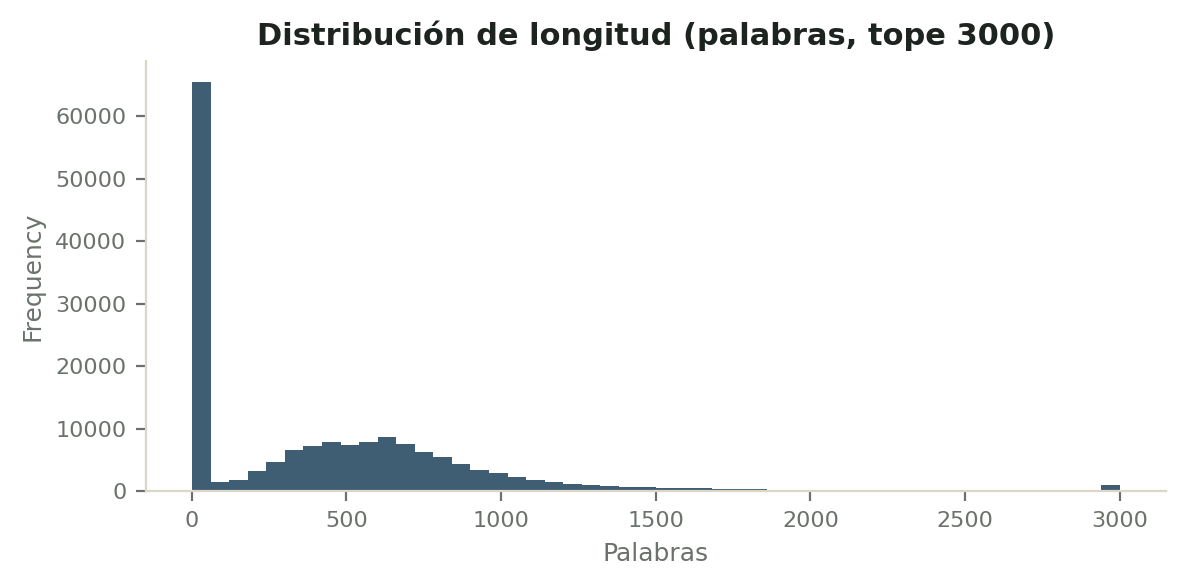
\includegraphics[width=0.8\textwidth]{perfil_longitud.png}
\caption{Distribuci\'on de longitud en palabras. Los documentos de m\'as de 3.000 palabras se acumulan en el extremo derecho del histograma.}
\label{fig:s4}
\end{figure*}



\section*{Progresi\'on de la configuraci\'on}

La Tabla~\ref{tab:progresion} resume el recorrido de la configuraci\'on: cada fila es una decisi\'on tomada con una medici\'on.

\begin{table}[H]
\centering
\footnotesize
\caption{Progresi\'on de la configuraci\'on y m\'etrica que la justific\'o.}
\label{tab:progresion}
\resizebox{\columnwidth}{!}{%
\begin{tabular}{lllll}
\toprule
Etapa & Cambio & Silver & M\'etrica & Decisi\'on \\
\midrule
Piloto & e5-base, 1.932 docs & piloto (38) & Recall@10 0,947 & Punto de partida \\
Escala & corpus completo & 38 & Recall@10 0,684 & El piloto sobreestima \\
Dispersa & BM25 & 38 & Recall@10 0,763 & No alcanza el techo \\
Codificador & bge-m3 & 38 & Recall@10 0,842 & Adoptado \\
\'Indice & \texttt{ef}=800 & 38 & Recall@10 0,895 & Adoptado \\
Fusi\'on & h\'ibrido RRF & 38 & Recall@10 0,895 & Empata, se descarta \\
Fusi\'on & h\'ibrido RRF & ampliado & Recall@10 0,890 & Rechazado \\
Reordenamiento & uni\'on densa+BM25 & reservado (20) & Recall@10 0,700 & Adoptado \\
Contexto & $k=10$ & reservado (20) & 19/20 entregadas & Adoptado \\
Prompt & v2 & 38 & 37/38 y cobertura 25/37 & Adoptado \\
Compuerta & 160 preguntas & 20 test & 0 falsos aceptados & Adoptado \\
Fase 6 & cuatro variantes & 38 & sin mejora & Rechazadas \\
Fase 7 & MMR & 38 & recall 0,816 & Rechazado \\
Reservado & 20 directas & reservado (20) & Recall@10 0,700 & Recupera parte de la ca\'ida \\
Compuerta & 5 negativas & reservado (5) & 5/5 rechazadas & 3/20 falsos rechazos \\
\bottomrule
\end{tabular}
}
\end{table}


\section*{Versiones de los modelos}

La Tabla~\ref{tab:modelos} fija la versi\'on de cada modelo. Los identificadores son las etiquetas de Ollama y de Hugging Face usadas en el c\'odigo. El checkpoint del reordenador es \texttt{BAAI/bge-reranker-v2-m3}; los artefactos no guardan un digest inmutable de cada modelo, as\'i que la etiqueta y la fecha de la corrida son la referencia disponible.

\begin{table}[H]
\centering
\footnotesize
\caption{Modelos, etiqueta y papel en el sistema.}
\label{tab:modelos}
\setlength{\tabcolsep}{3pt}
\begin{tabular}{lll}
\toprule
Papel & Etiqueta & Cuantizaci\'on \\
\midrule
Generador & \texttt{gemma4:e4b} & Q4\_K\_M \\
Condensador y juez & \texttt{gemma2:2b} & Q4\_K\_M \\
Embedding & \texttt{BAAI/bge-m3} & fp16 en GPU \\
Reordenador & \texttt{BAAI/bge-reranker-v2-m3} & fp16 en GPU \\
Comparaci\'on E4 & \texttt{qwen2.5:1.5b} & Q4\_K\_M \\
Comparaci\'on E4 & \texttt{llama3.2:3b}, \texttt{llama3.2:1b} & Q4\_K\_M \\
Comparaci\'on E3 & \texttt{qwen3-embedding:8b} & Q4\_K\_M \\
\bottomrule
\end{tabular}
\end{table}


\end{document}
